\documentclass{article}
\usepackage{float}
\usepackage{enumitem}
\setenumerate[1]{itemsep=0pt,partopsep=0pt,parsep=\parskip,topsep=5pt}
\setitemize[1]{itemsep=0pt,partopsep=0pt,parsep=\parskip,topsep=0pt}
\setdescription{itemsep=0pt,partopsep=0pt,parsep=\parskip,topsep=5pt}
\usepackage{enumerate}
\usepackage{geometry}
\geometry{verbose,tmargin=0.07\paperheight,bmargin=0.07\paperheight,lmargin=0.1\paperwidth,rmargin=0.1\paperwidth}
\usepackage{graphicx} 
\usepackage{hyperref}
\usepackage{hyperref}
\hypersetup{
    colorlinks=true,
    citecolor=blue,
    linkcolor=blue,
    urlcolor=blue
}
\usepackage{indentfirst}
\usepackage[round]{natbib}
\usepackage{booktabs}


\setlength{\bibsep}{0.0pt}
\setlength{\parindent}{2em}

\makeatletter         
\def\@maketitle{
\newpage
\null
\vskip -2em 
\begin{center}
\let \footnote \thanks
{\LARGE \@title \par}
\vskip .5em
{\large
 \lineskip .5em
\begin{tabular}[t]{c}
    \@author
\end{tabular}\par}
\vskip .5em
{\large \@date}
\end{center}
\par
\vskip .5em}
\makeatother

\newcommand{\eg}{\textit{e}.\textit{g}. }

\title{Music Transcription and Generation}

\begin{document}

\maketitle

\begin{abstract}
    This paper presents a novel paradigm for generating music pieces from short multi-track recordings. To overcome the complexity of processing audio waves and the high data volume, we transform musical features into a MIDI-encoded format.
\end{abstract}

\section{Introduction}

The application of deep learning in music research is motivated by several factors. Primarily, music, like language, is a form of sequential data with complex, hierarchical structures. Deep learning models, such as Recurrent Neural Networks (RNNs) and Transformers, have proven to be highly effective in understanding such data structures, making them a promising tool for music analysis. Moreover, deep learning can facilitate tasks like music generation, classification, and recommendation by learning to recognize patterns and structures in music data that are difficult for humans to discern. 

For instance, deep learning models can generate new music by learning from a large dataset of songs, or they can classify music into genres by recognizing subtle patterns in the music's features. We focus on the another interesting question is that how to generate a longer piece of music from a multi-track raw music segment, which complies with basic music theory and can also be appreciated by human.

Our goal is to design a new paradigm (\autoref{fig:paradigm}) for music generation. Firstly, we employ a transcription head to capture musical aspects and encode them into a MIDI file. This MIDI file, which is packed with priors, is then used as the input for the subsequent generation model. 

\begin{figure}[H]
    \centering
    
\includegraphics[scale=0.4]{Figure/paradigm.png}
    \caption{New paradigm for music generation.}
    \label{fig:paradigm}
\end{figure}

The motivations for this circuitous approach are desired to overcome the following challenges:

\begin{itemize}
\item [$\diamond$] Musical waves are highly complex and compressed forms of data, incorporating various aspects such as melody, harmony, rhythm, and timbre (different instruments). Models that generate music based on these data are difficult to capture all musical aspects.
\item [$\diamond$] Wave files contain huge data per second, which will make the model heavy and require significant computational resources.
\item [$\diamond$] Real-world music is typically captured and stored as audio files. Therefore, relying solely on MIDI files for music representation and generation may not align with practical settings.
\item [$\diamond$] For long musical sequences, the application of efficient compression and encoding methods is crucial to reduce memory requirements and training complexity.
\end{itemize}

\section{Related Works}
Whether it's classification, separation, transcription or generation, early methods of processing audio with machine learning primarily relied on techniques from computer vision. Later, with the development of NLP tasks, attempts were made to introduce sequential models and attention mechanisms into audio, which also has sequential properties.

\subsection{Classification/Separation}

Classification and separation are two common tasks in music processing that use machine learning techniques to analyse and manipulate musical data. The classification task aims to identify the instrument or emotion of a musical piece by extracting spectral features from the audio signal, while the separation task attempts to separate a mixed track into multiple independent instrument tracks by applying multi-channel learning methods.

One of the representative works in this area is Wave-U-Net \citep{stoller2018waveunet}, which is a modified version of the U-Net architecture that performs multi-scale analysis of music signals through 1D-convolution and downsampling layers. Other researchers have adopted sequence-based models 
by treating music as a text-like sequence of information and using network architectures such as RNNs or Transformers to extract features from it. Some successful examples of this approach are the Open-Unmix \citep{stoter2019open} model, which uses a three-layer LSTM network, and the Demucs \citep{defossez2020real} model, which combines transformer and U-Net architectures.

\subsection{Transcription}

Music transcription is a task that converts audio signals into symbolic representations (such as MIDI file or scores), which can be used for music analysis, education, composition, and other fields. In recent years, with the help of deep learning algorithms, the accuracy and efficiency of music transcription task has achieved some significant progress and results.

Traditional algorithms use dynamic programming algorithms based on hidden Markov models (HMMs) to process the spectral features of audio, and calculate the pitch probability distribution of each time frame, but the results are generally poor. Some researchers considered the Markov property of audio signals, and combined convolutional neural networks (CNNs) and recurrent neural networks (RNNs) to extract spectral features, achieving improved accuracy in this field \citep{9413601}. However, under more tracks and more complex acoustic conditions, such as considering harmony, polyphony, resonance, etc., the performance of RNN-based models is still very limited.

Recent research aims to use more powerful attention-based sequence models for music transcription. The initial model is a generic encoder-decoder Transformer \citep{hawthorne2021sequence}. This model takes as input a random audio segment, processed by the Short Time Fourier Transform (STFT) and scaled to a Mel spectrogram. The model's output at each step is a softmax distribution over a discrete vocabulary of events. Researchers made the vocabulary to fit the MIDI specification messages, adapting the task to the Transformer architecture. In a subsequent study \citep{gardner2021mt3}, the model was extended for multi-track music transcription by incorporating instrument tokens into the vocabulary. And they proposed several useful metrics for evaluating multi-instrument transcription models.

\subsection{Generation}
The generation of music can be broadly divided into two categories: one employs more traditional methods such as Convolution Neural Networks (CNNs) and RNNs, while the other leverages Transformer models. A representative of the former category is WaveNet \citep{oord2016wavenet}, which captures long-term relationships by employing dilated causal convolutions to expand the receptive field, offering the advantage of low computational resource requirements. An example of the latter category is MuseNet, which is based on the Sparse Transformer \citep{child2019generating}. 

However, music is not just sequential data; it also has symbolic features. Models that account for these features are expected to yield better performance.

Symbolic music generation refers to the process of creating music represented as a series of symbols. \citep{Todd} initially used an RNN to predict the pitch and duration of notes, generating monophonic music one note at a time. However, RNNs face challenges such as vanishing and exploding gradients when handling long musical sequences.

Building on the robust structures offered by Transformers, more research has shifted towards addressing the second challenge:  model complex musical sequence representations, such as multi-track compositions. MMM \citep{ens2020mmm} condenses multiple tracks into a single, time-ordered sequence of musical events. However, the use of time-delta tokens and fixed positional encoding in MMM weakens the correlation and structure between tracks at the note level. The recently proposed SymphonyNet\citep{liu2022symphony} introduces the Multi-track Multi-instrument Repeatable (MMR) representation, based on the semi-permutation invariant in musical scores, and employs the novel Music BPE to reduce the input sequence length, offering better solutions for both challenges.

\section{Problem Definition}

\subsection{Dilemma between efficiency and effectiveness in transcription} 

A large number of studies have shown a dilemma in the music transcription task. When we try to serialize the spectral features of the audio, the length of the sequence can reach the order of millions, and even for a single syllable, its length can reach the order of thousands. It is difficult to extract features from such a long sequence, especially in the attention-based sequence models that are sensitive to length. Unfortunately, in the music transcription task, the overall features of the sequence are important, and methods such as reducing the sampling rate to reduce length of the sequence will lead to a decline in model performance. Therefore, how to extract features of the serialized spectrum efficiently is a problem to be solved.

\subsection{Deficiency in SymphonyNet} 

The SymphonyNet has introduced lots of novel approaches for processing musical series data in order to do music generation. However, the model has certain limitations. First, it employs a linear attention mechanism, which, while computationally less demanding, results in lower training efficiency of the model. The authors have integrated an recurrent structure into the inference framework to save the space and improve the processing velocity. But this design diverges from the conventional method of inference, which typically relies on self-autoregression.

Additionally, the evaluation doesn't account for variations in the length of the music data provided, which is an important factor to consider when assessing the model's performance under different circumstances.

\section{Approach}

\subsection{From audio to MIDI}

As we discussed in previous sections, before the music generation task, we need to transcribe the audio files into MIDI format, to obtain the tokenized sequence that is easier to process and has more obvious features.

As shown in Figure ~\ref{transcription}, We divide the whole transcription process into three steps:

\begin{figure}[H]
	\centering
        \vspace{-0.3cm}
	\centerline{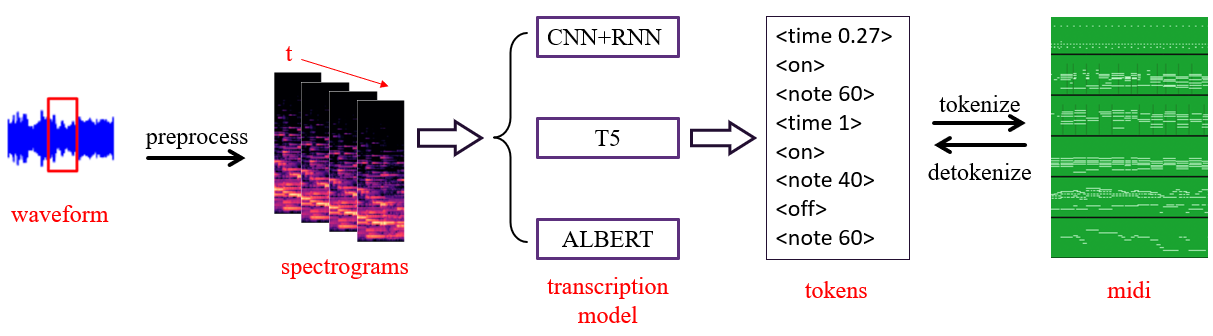
\includegraphics[width=13cm]{Figure/transcription.png}}
        \vspace{-0.25cm}
	\caption{The data processing workflow from audio files to MIDI files.}
        \label{transcription}
\end{figure}

\begin{enumerate}
    \item Convert the waveform audio data into spectrograms using Fourier Transform or other frequency analysis algorithms. 
    \item Use deep learning models to extract features from spectrograms. Three kinds of model are considered: the traditional RNN model with convolutional layers, the Text to Text model represented by T5, and the Encoder-only model represented by Albert.
    \item Organize tokens obtained by model inference and output MIDI files. After defining the correspondence between tokens and MIDI file symbols, we can also convert MIDI files back to tokens.    
\end{enumerate}

\subsection{Our generation pipeline}
Although SymphonyNet has achieved significant success in the generation of multi-track music, we've identified several issues within its framework. The linear transformer, serving as the framework's backbone, requires improvements in both generation efficiency and effectiveness. Additionally, the relative position encoding employed during the encoding stage lacks essential information about the model's positional context. 
Furthermore, upon careful review of the code, it was noted that the model employs distinct architectural designs during training and inference phases: a linear transformer for training, and a recurrent transformer for inference. While efficient in terms of time and space, this approach struggles to model correlations effectively in longer sequences.

\begin{figure}[H]
	\centering
        % \vspace{-0.3cm}
	\centerline{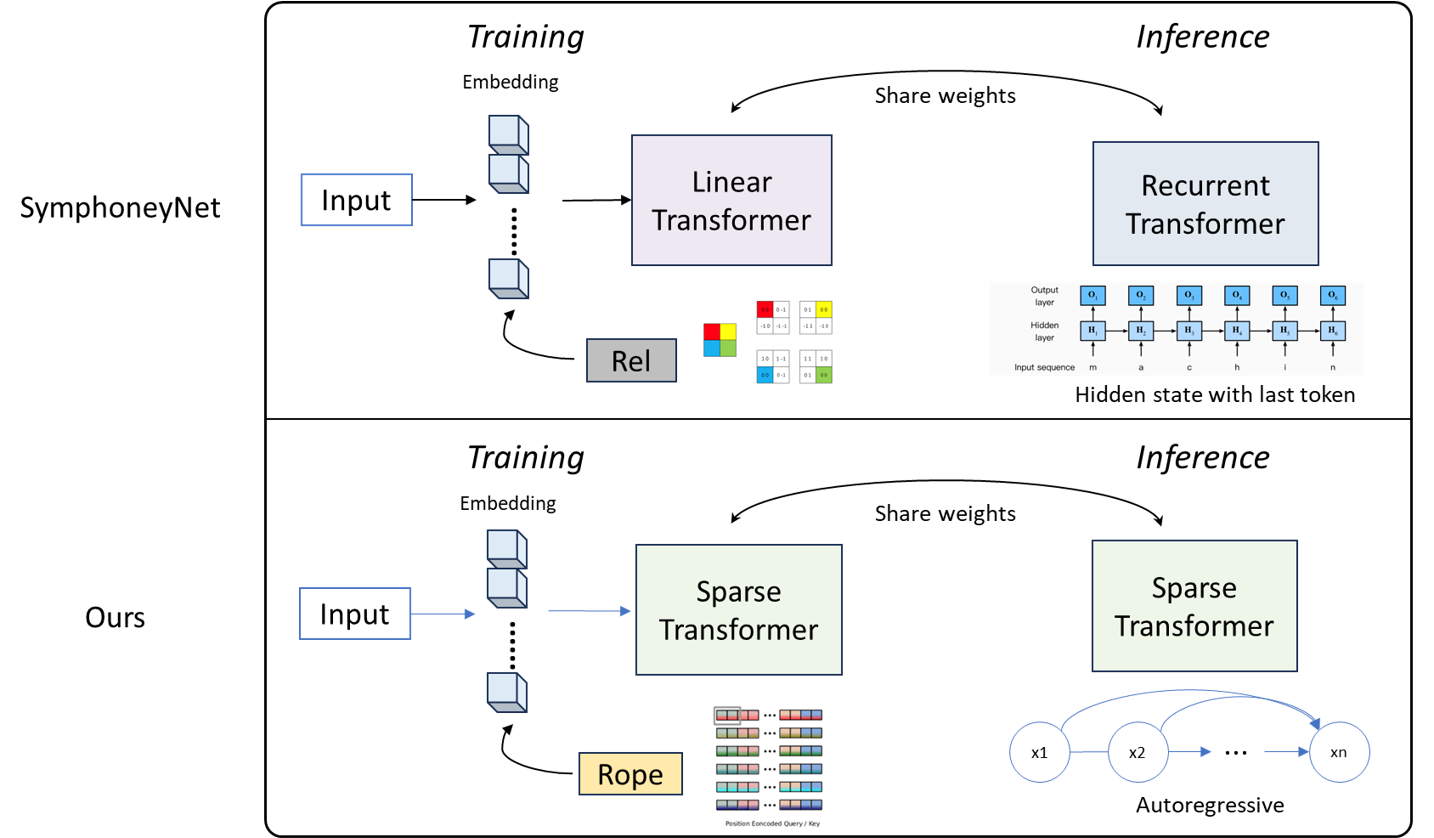
\includegraphics[width=13cm]{Figure/modification pipeline.png}}
	%  \vspace{2.0cm
        %\vspace{-0.2cm}
        % \captionsetup{belowskip=0pt}
        % \vspace{-0.25cm}
	\caption{The overall framework of our proposed generation pipeline with the modification over SymphonyNet in training and inference procedures.}
        \label{Geneation framework}
        % \vspace{-0.25cm}
\end{figure}

Therefore, to tackle the problems above, we propose a refined framework designed to standardize music generation more effectively.
Figure~\ref{Geneation framework} illustrates the design of our proposed framework, which is based on a sparse transformer~\cite{sparse} and highlights the technical differences between our approach and SymphonyNet. 
Our enhancements focus primarily on the training and inference stages. In the training stage, we transition from a linear to a sparse transformer.
Additionally, we introduce rotary position embedding (rope)~\cite{rope} to integrate absolute and relative position encoding. Compared to the relative position embeddings used in SymphonyNet, rope offers a more flexible method for encoding positional information, which can capture the relationships within a sequence more accurately.

For inference, our framework maintains architectural consistency between the training and inference phases, employing a standard autoregressive approach for generating music sequences. This autoregressive method generates sequences based on the preceding tokens, thereby capturing a more nuanced and contextually rich semantic information.

\section{Experiments}

\subsection{Experiment Setup} 
\subsubsection{Datasets}
For music transcription, MAESTRO dataset is chosen for training and testing.The dataset contains about 200 hours of paired audio and MIDI recordings from ten years of International Piano-e-Competition. Audio and MIDI files are aligned with ∼3 ms accuracy and sliced to individual musical pieces, which are annotated with composer, title, and year of performance. 

For multi-track music generation, We evaluate the performance on Symphony Dataset~\citep{liu2022symphony}, which comprises over 46,000 online symphonic music MIDI files with an average duration of 4.26 minutes. This dataset stands as one of the few foundational, symbolic multi-track music datasets worldwide. Following~\citep{liu2022symphony}, the split ratio for the training, validation, and test sets is set to 8:1:1.

\subsubsection{Implementation Details} In this paper, three transcription models have been trained and tested， which are a hybrid architecture combining recurrent neural network and convolutional neural network, T5 model, and Albert model.The architecture of previous two models are the same as those reported by ~\citep{9413601} and ~\citep{gardner2021mt3}.We also built an Albert based model with 12 hidden layers and input length of 512 for its less parameters.

As for the generation model, we train a sparse transformer~\citep{sparse} decoder model as the backbone, which adopts 4096 as the length of input sequence, with a fixed sparse window size of 16. We set the embedding size for event tokens, durations, instruments and 3-D positional embedding to 512.
The batch size is set to 128 and the model is optimized across 10 epochs using a base learning rate of 0.0003, employing the Adam optimizer for this purpose.
In the preliminary phase of training, we established a regimen of 10,000 steps of warm updates to gradually adapt the learning rate, ensuring a more stable and efficient convergence of the model's parameters.


\subsubsection{Baselines} To evaluate the effectiveness of our improved model in the multi-track music generation, we make comparisons our counterpart SymphonyNet~\citep{liu2022symphony} and the popular music tool Continue~\citep{magentastudio}, developed by Google's Magenta project.

\subsubsection{Metrics} 
Frame metric and onset metric are chosen to evaluate our transcription results. Frame metrics compare the prediction and target results frame by frame and calculate the F1 score while onset metrics focus on the beginning of a certain note and calculate the F1 score with tolerance, which means that the time error and pitch error in a certain range will be accepted. 

Owing to the fact that the majority of music generation evaluations predominantly employ human assessment, we find ourselves constrained by a lack of requisite resources to undertake such evaluations. Consequently, we will not incorporate the human-varified metric in our baseline comparisons. 
However, to scrutinize the impact of various parameters on our model, we will adopt a 5-dimensional scoring method akin to that used by [xxx] in our ablation studies and model analysis experiments.
The generation samples will be assessed across five dimensions: Coherence (C), Diversity (D), Harmoniousness (H), Structureness (S), Orchestration (O) and Overall Preference (P), in a 5-point Likert scale.

\subsection{Performance evaluation}
\subsubsection{Performance of transcription}
In table \ref{onset_result} and \ref{frame_result}, we show the metrics of different models. Due to the submission deadline constraints, the Albert model has not been tested yet and the training process has been completed with the loss curve shown in Figure \ref{albert_loss}.
\begin{table}[H]
    \centering
    \begin{tabular}{cccc}
        \hline
         model &  onset F1 & onset precision & onset recall\\
         \hline
         RNN-CNN &  - & - & - \\
         T5 & 0.9712 & 0.9927 & 0.9510 \\
         \hline
    \end{tabular}
    \caption{onset metrics of different models}
    \label{onset_result}
\end{table}

\begin{table}[H]
    \centering
    \begin{tabular}{cccc}
        \hline
         model &  Frame F1 & Frame precision & Frame recall\\
         \hline
         RNN-CNN &  0.2686 & 0.2195 & 0.9061\\
         T5  &  0.6157 & 0.4860 & 0.9179 \\
         \hline
    \end{tabular}
    \caption{Frame metrics of different models}
    \label{frame_result}
\end{table}

\begin{figure}[H]
    \centering
    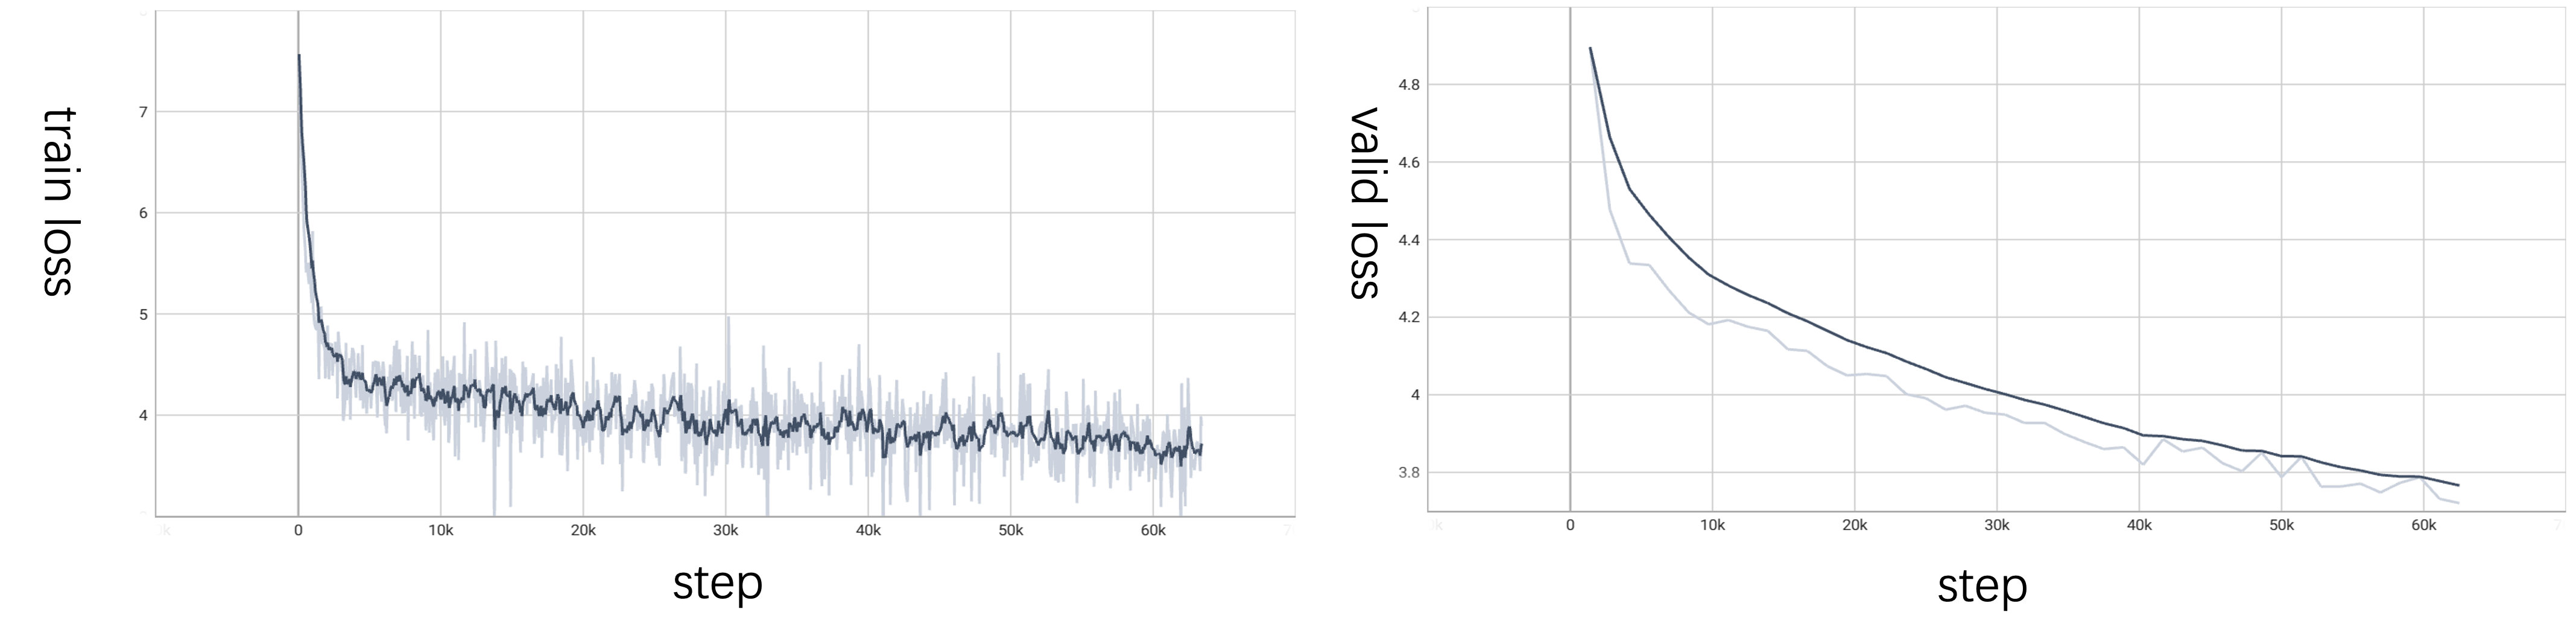
\includegraphics[width=0.9\textwidth]{Figure/albert_loss.png}
    \caption{Training (left) and validation (right) curves of our albert model}
    \label{albert_loss}
\end{figure}
We also plot the pianoroll of our transcription results. Figure \ref{oianoroll_a2s} shows the predicting result of RNN-CNN model. Most beginnings of musical notes can  be correctly predicted, but gaps frequently occur in the middle of a note.The visual result indicates that frame metrics is lower than the onset metrics, which is consistent with the numerical results above. On our dataset, tranformer-based model performs much better than the model based on RNN and CNN.
\begin{figure}[H]
	\begin{minipage}[t]{0.46\linewidth}
		\centering
		\centerline{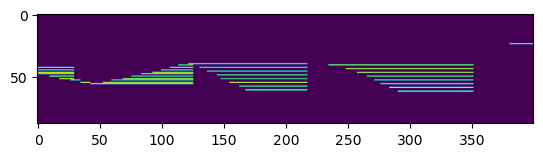
\includegraphics[width=2.8in]{Figure/a2s_target.png}}
		% \centerline{(a)}\medskip
	\end{minipage}
	\hfill
	\begin{minipage}[t]{0.46\linewidth}
		\centering
		\centerline{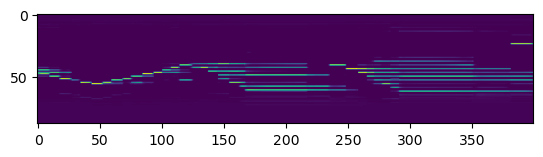
\includegraphics[width=2.8in]{Figure/a2s_pred.png}}
		% \centerline{(b)}\medskip
		%  \vspace{2.0cm}
	\end{minipage}
	%
 	% \caption{Schematics of contrastive gradient regularization. (a) If the average gradient of the semantic regulator does not align with the positive, the negative gradients will not be changed. 
  %     (b) Otherwise, regularization will be applied to the negative gradients to diverge positive and negative gradient directions.}
        \vspace{-0.1cm}
       \caption{Target pianoroll (left) and prediction pianoroll (right) curves of RNN-CNN model.}
        \label{oianoroll_a2s}
\end{figure}
Two example generated by T5-based model are shown as follows.Blue, cyan and light green represent for True Positive, False Negative and False Positive separately.
\begin{figure}[H]
    \centering
    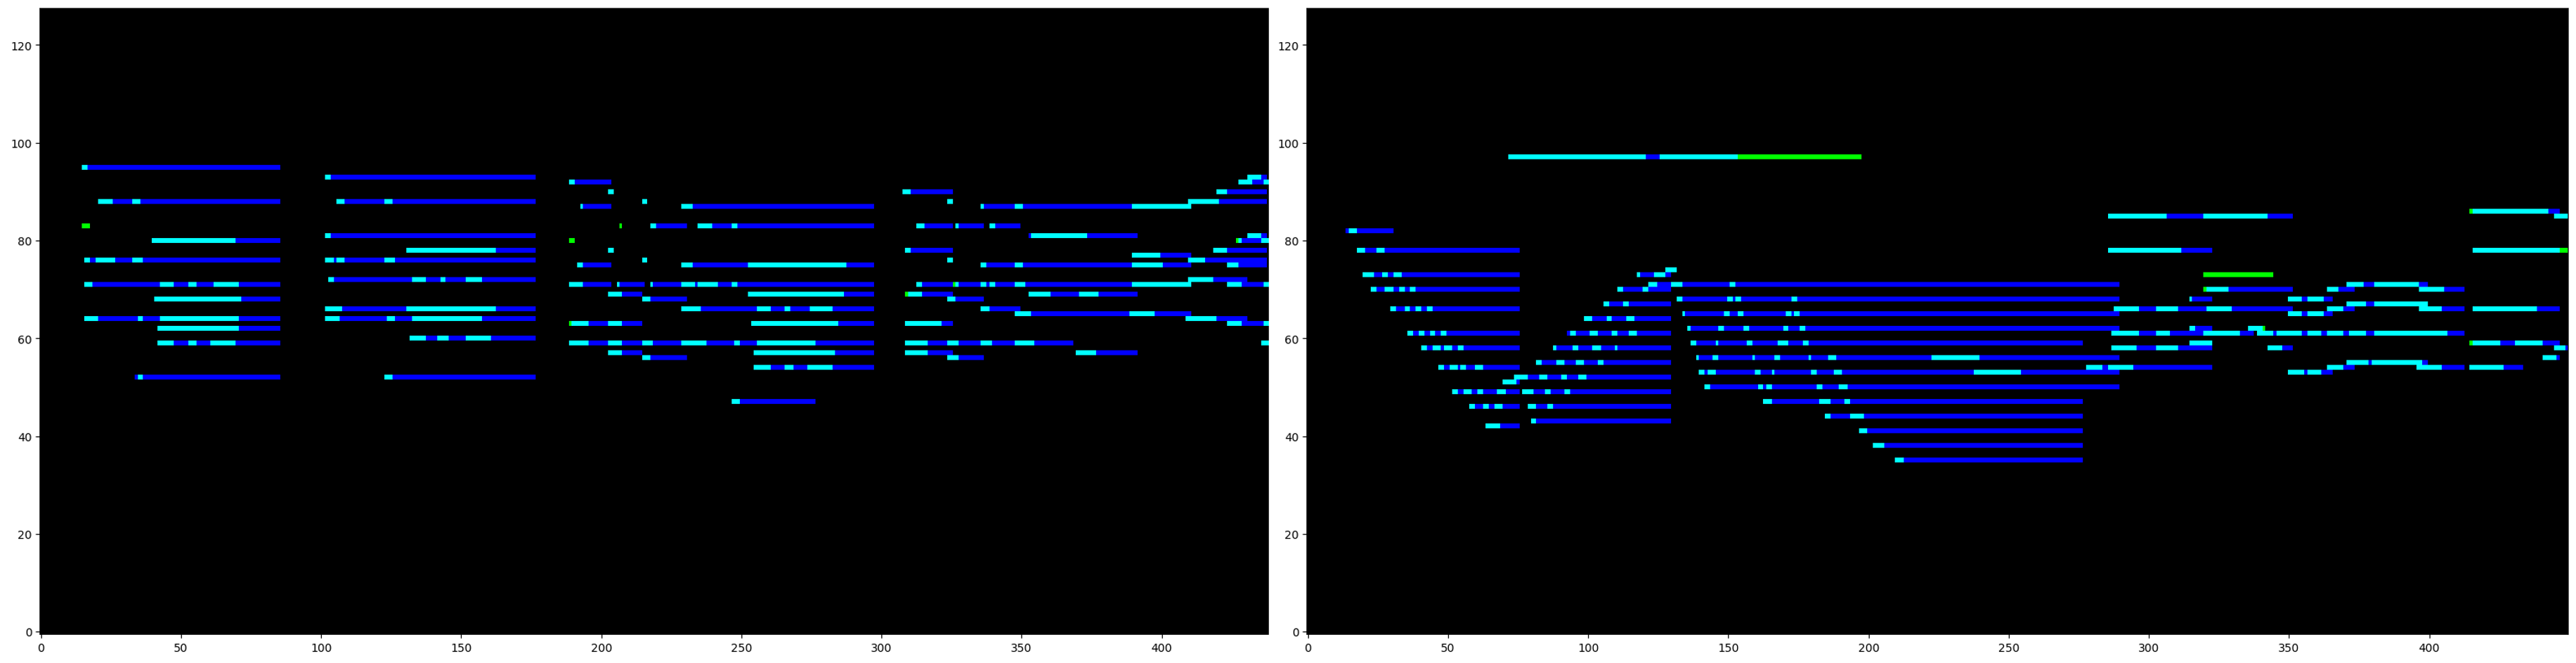
\includegraphics[width=0.9\textwidth]{Figure/result_T5.png}
    \caption{two examples generated by T5}
    \label{output_T5}
\end{figure}
\subsubsection{Performance of generation}
\begin{figure}[H]
	\begin{minipage}[t]{0.46\linewidth}
		\centering
		\centerline{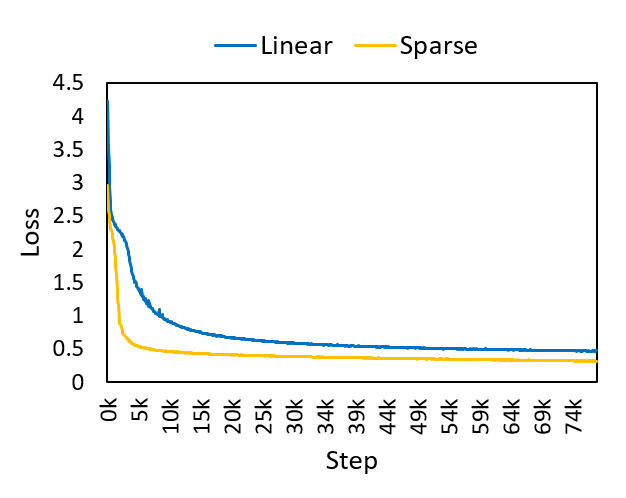
\includegraphics[width=2.8in]{Figure/train_curve_comp1.png}}
		% \centerline{(a)}\medskip
	\end{minipage}
	\hfill
	\begin{minipage}[t]{0.46\linewidth}
		\centering
		\centerline{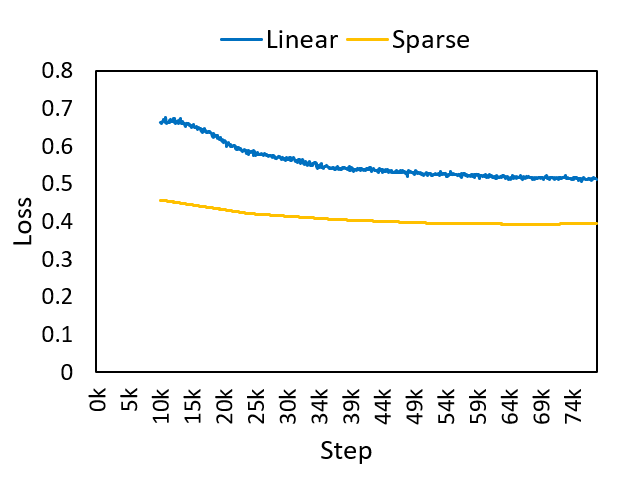
\includegraphics[width=2.8in]{Figure/valid_curve_comp1.png}}
		% \centerline{(b)}\medskip
		%  \vspace{2.0cm}
	\end{minipage}
	%
 	% \caption{Schematics of contrastive gradient regularization. (a) If the average gradient of the semantic regulator does not align with the positive, the negative gradients will not be changed. 
  %     (b) Otherwise, regularization will be applied to the negative gradients to diverge positive and negative gradient directions.}
        \vspace{-0.1cm}
       \caption{Training (left) and validation (right) curves of different attention paradigm.}
        \label{fig: curves}
\end{figure}

\begin{figure}[H]
	\centering
        \vspace{-0.3cm}
	\centerline{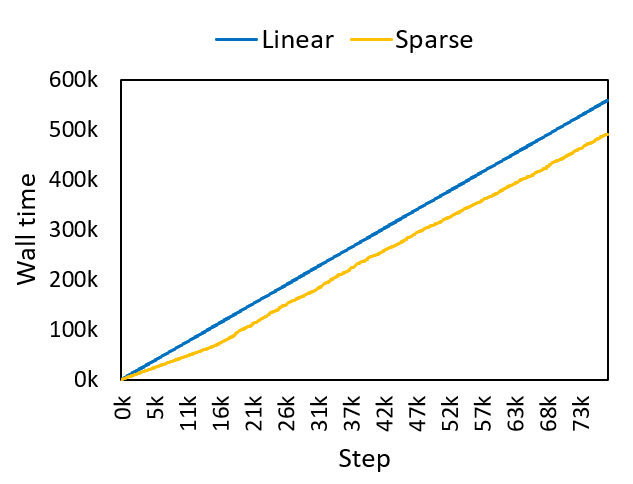
\includegraphics[width=7cm]{Figure/time_comp1.png}}
	%  \vspace{2.0cm
        %\vspace{-0.2cm}
        % \captionsetup{belowskip=0pt}
        \vspace{-0.25cm}
	\caption{Comparison on training wall time.}
        \label{wall time}
        \vspace{-0.25cm}
\end{figure}


In Figure~\ref{fig: curves}, the yellow line illustrates the improvements in both the convergence speed and loss reduction that our sparse attention model achieves compared to the original SymphonyNet (blue).
As shown, our model nearly reaches a state of stable convergence at nearly 5k step during training, while SymphonyNet attains a similar level of stable convergence around the 40k step, which is eight times longer than ours.

Simultaneously, the training wall time, as shown in Figure~\ref{wall time}, further demonstrates the high efficiency of our sparse transformer decoder. With a more gradual slope, our model requires less training time for the same number of training steps.

\begin{figure}[H]
	\begin{minipage}[t]{0.46\linewidth}
		\centering
		\centerline{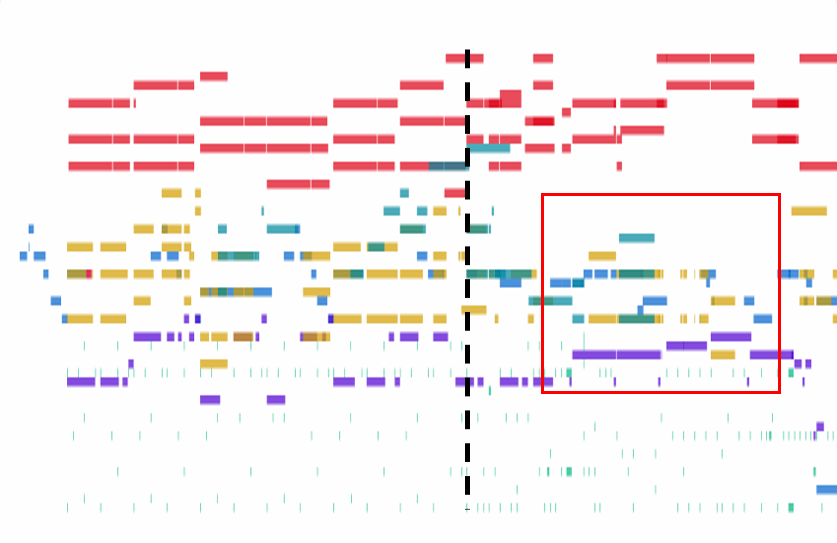
\includegraphics[width=2.5in]{Figure/ours_generation.png}}
		\centerline{(a) Ours}\medskip
	\end{minipage}
	\hfill
	\begin{minipage}[t]{0.46\linewidth}
		\centering
		\centerline{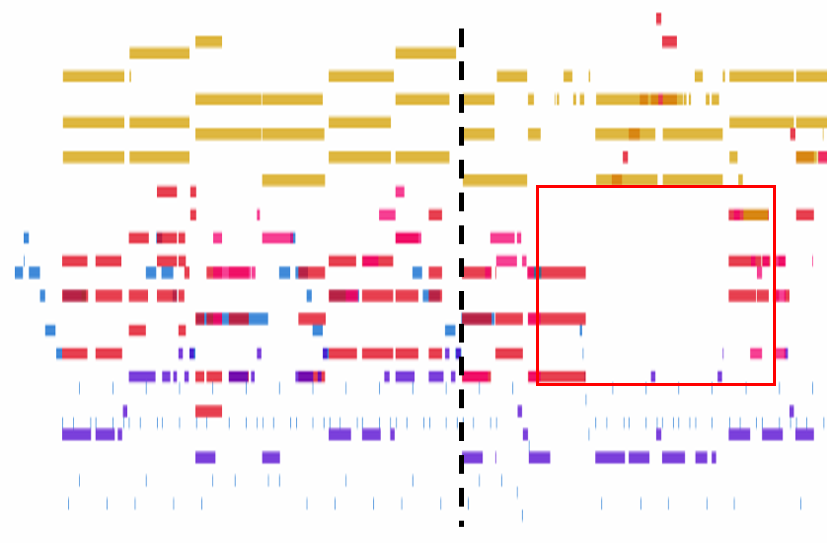
\includegraphics[width=2.51in]{Figure/continue_generation.png}}
		\centerline{(b) Continue}\medskip
	  % \vspace{0.7cm}
	\end{minipage}
	%
        
       \caption{Visualization comparison between ours and Continue~\cite{magentastudio}.}
        \label{fig: continue}
\end{figure}


% Regarding generation effectiveness, as mentioned in our presentation, we observed that SymphonyNet employs the RNN during inference yields better results when the size of conditional tokens is relatively low. However, as the number of input conditional tokens increases, its generative performance progressively deteriorates.
In terms of generative effectiveness, as mentioned in our presentation, we observed that SymphonyNet's recurrent transformer during inference yields better results when the size of the conditional tokens is relatively small (\eg $token=5$). Conversely, our model underperforms when the number of conditional tokens is limited, but its generative capabilities improve as their size increases. The experiment results indicate that our model, with the standard autoregressive mode, is more adept at modeling dependencies in longer sequences (\eg $token \geq 10$), while the inference mode of SymphonyNet is more suited to scenarios requiring rapid music generation and those with a smaller number of token conditions. 
However, from the standpoint of model evaluation, we do not advocate using different model architectures during training and inference. Such an approach hinders the analysis for the efficacy of individual model components, thereby obstructing potential enhancements in performance.

To further demonstrate the superiority of our model, we conduct a comparative analysis with a currently popular music processing tool, Continue~\citep{magentastudio}, developed by Google's team. As shown in Figure~\ref{fig: continue}, our model outperforms Continue in terms of the complexity of the generated music, which indicates that our model's enhanced capabilities in handling multi-track music generation.

\section{Insights Analysis}

\subsection{Transcription Model}

The models we considered in the data workflow actually correspond to three ways of understanding the transcription task. The RNN model with convolutional layers assumes that the pitch and intensity of the audio are mainly determined by the local distribution of the spectrograms. The T5 model treats the transcription task as a translation task, trying to “translate” the spectrograms into a musical language represented by the MIDI format. The Albert model transforms the transcription task into a token-classification task, believing that the model can learn sequence features and convert the spectrograms into tokens frame by frame by classification.

The experiments show that the transcription model performs well near the onset of notes, and can accurately identify the pitch, intensity, and relative position. In the T5 model, the accuracy reaches over 99\%. 

We noticed that the RNN model has a mediocre performance in recognizing the note duration and the pitch variation during the note sustain, which may be due to its weak ability to extract overall features of the sequence, and its accuracy is only 26\%. The T5 model has improved in this aspect, and its accuracy has reached 60\%. In fact, acoustic studies show that human ears are not sensitive to the audio changes during the note sustain, while the main way for humans to identify music is based on the type and position of the notes. Therefore, with 99\% accuracy of note position and 60\% accuracy of note sustain, the transcription result sounds almost identical to the original audio.

\subsection{Generation Model}
\begin{figure}[H]
	\begin{minipage}[t]{0.46\linewidth}
		\centering
		\centerline{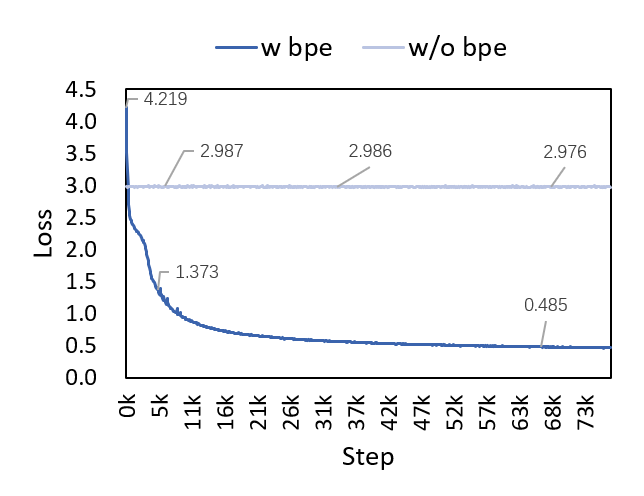
\includegraphics[width=2.8in]{Figure/train_curve_comp2.png}}
		% \centerline{(a)}\medskip
	\end{minipage}
	\hfill
	\begin{minipage}[t]{0.46\linewidth}
		\centering
		\centerline{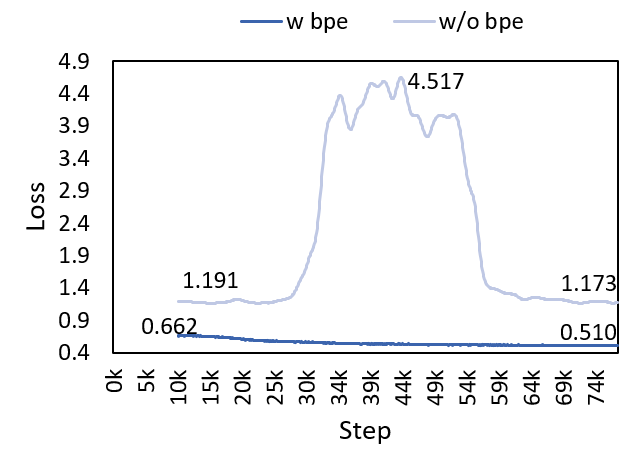
\includegraphics[width=2.85in]{Figure/valid_curve_comp2.png}}
		% \centerline{(b)}\medskip
	  % \vspace{0.7cm}
	\end{minipage}
	%
 	% \caption{Schematics of contrastive gradient regularization. (a) If the average gradient of the semantic regulator does not align with the positive, the negative gradients will not be changed. 
  %     (b) Otherwise, regularization will be applied to the negative gradients to diverge positive and negative gradient directions.}
        % \vspace{-0.5cm}
       \caption{Training (left) and validation (right) curves of SymphonyNet with respect to Music BPE.}
        \label{fig: curves2}
\end{figure}

\begin{figure}[H]
	\centering
        % \vspace{-0.3cm}
	\centerline{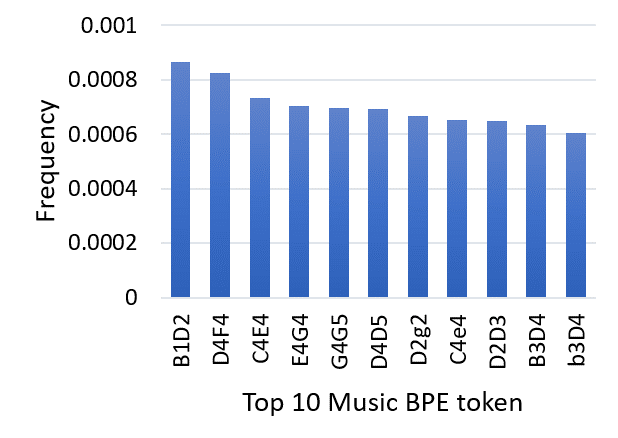
\includegraphics[width=7cm]{Figure/music BPE.png}}
	%  \vspace{2.0cm
        %\vspace{-0.2cm}
        % \captionsetup{belowskip=0pt}
        % \vspace{-0.25cm}
	\caption{Music BPE note aggregation results.}
        \label{music bpe}
        
\end{figure}


\textbf{Ablation study on Music BPE. } We have verified the effectiveness of Music BPE as proposed in SymphonyNet. As shown in Figure~\ref{fig: curves2}, during the training of the baseline, the curve fails to converge without Music BPE. Moreover, Figure~\ref{fig: curves2}(right) shows an uncontrollable rise in validation loss without Music BPE. Conversely, there is a discernible slight downward trend in the validation loss with Music BPE. The results clearly demonstrates that this technique is indispensable in this project. 

Following SymphonyNet, we have illustrated the results of Music BPE note aggregation in Figure~\ref{music bpe}. It is evident that the aggregated number of notes occupies a considerable proportion throughout the entire sequence. After applying Music BPE to the whole music corpus, the average token length of a music piece reduces from \textbf{2.28} to \textbf{1.13}.

% Table generated by Excel2LaTeX from sheet 'Sheet1'
\begin{table}[H]
  \centering
  \caption{Human evaluation for different token number in conditional generation.}
  \vspace{0.5cm}
    \begin{tabular}{ccccccc}
    \toprule
    \textbf{Cond. Tokens} & \textbf{C} & \textbf{D} & \textbf{H} & \textbf{S} & \textbf{O} & \textbf{P} \\
    \midrule
    5     & 1.79  & 1.54  & 2.21  & 2.43  & 3.32  & 2.26  \\
    10    & 2.41  & 3.41  & 3.50  & 2.29  & 2.43  & 2.81  \\
    15    & \textbf{2.53}  & \textbf{3.32}  & \textbf{3.62}  & 2.67  & 2.52  & 2.93  \\
    20    & 2.51  & 3.20  & 3.57  & \textbf{2.91}  & \textbf{2.60}  & \textbf{2.96}  \\
    \bottomrule
    \end{tabular}%
  \label{evaluate}%
\end{table}%

\textbf{Analysis on the conditional tokens. }To evaluate the optimal length of input sequences for better results, we compare the quality of generated music excerpts from various input lengths. We randomly selecte 10 MIDI files and analyze them across varying lengths of conditional tokens. The final outputs are evaluated based on the established evaluation metrics, with the results presented in Table~\ref{evaluate}.

\begin{figure}[H]
	\begin{minipage}[t]{0.46\linewidth}
		\centering
		\centerline{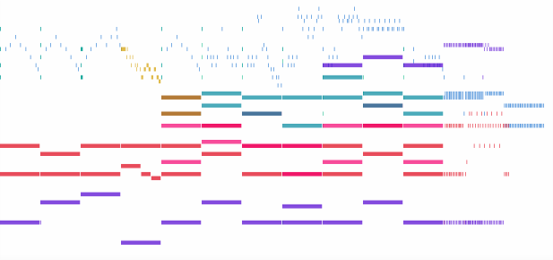
\includegraphics[width=2.8in]{Figure/w_mask.png}}
		\centerline{(a) With mask.}\medskip
	\end{minipage}
	\hfill
	\begin{minipage}[t]{0.46\linewidth}
		\centering
		\centerline{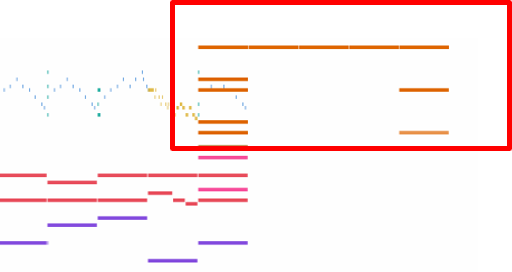
\includegraphics[width=2.6in]{Figure/w_o_mask.png}}
		\centerline{(b) Without mask.}\medskip
	  % \vspace{0.7cm}
	\end{minipage}
	%
        
       \caption{Impact of decoder mask.}
        \label{fig: mask}
\end{figure}

\textbf{Effect of decoder mask. } % We discovered that in autoregressive generation, the decoder mask significantly impacts the quality of generation, as illustrated in the Figure~\ref{fig: mask}. It enhances the diversity of the generated music. Without the mask, the generation process tends to produce prolonged periods of monotonous tones.
In Figure~\ref{fig: mask}, we explore the impact of the decoder mask on the quality of music generation, as demonstrated via track visualization. The absence of the mask results in a tendency for the generated music to fall into a pattern of prolonged monotonous tones. Therefore, the decoder mask is crucial in ensuring the continuity and diversity of the generated compositions.


\section{Conclusion}
For music transcription, we constructed a general framework for transcription tasks, utilizing the sequence processing capabilities of transformers to transcribe audio files into MIDI files, which is similar to text translation.  Despite problems such as note discontinuity in our model, it can provide a good foundation for subsequent music generation work.
For music generation, modifications to the attention mechanism, the position embedding method and the inference structure contribute to faster convergence during model training, as detailed in Section 5. Compared to the well known Magenta Continue tool, our model demonstrates significantly better performance in generating multi-track music, whereas Continue is limited to producing simpler, single-track music.

For future work, we plan to employ a transfer learning approach to train our model on datasets transcribed by the transcription model. This strategy is expected to better align with the real-world scenarios where we initially obtain raw audio data.

\bibliographystyle{apalike}
\bibliography{bibliography}
\end{document}
